\documentclass[12pt,a4paper]{article}

% Quelques options d'encodage, de langues et de format du document
\usepackage[utf8]{inputenc}
\usepackage[T1]{fontenc}
\usepackage[english]{babel}
\usepackage[top=2cm, bottom=3cm, left=1.75cm, right=1.75cm]{geometry}
\usepackage{setspace}

\usepackage{graphicx} % Pour la commande "\includegraphics"
\usepackage[ % Modified parameters
    bookmarks,
    colorlinks,
    citecolor=black,
    urlcolor=blue,
    linkcolor=black,
    pdfpagemode=UseNone
]{hyperref} % Pour la commande "\url"

\pagenumbering{arabic}

% ------------------------------------------------------------------
% CITATION MANAGEMENT
% ------------------------------------------------------------------

% APA Style
\usepackage{cite}
%\bibliographystyle{apalike}
\bibliographystyle{ieeetr}

\renewcommand\refname{Bibliography}

% Proper formatting and line breaking for URLs
\usepackage{url}

% Change "References" to "Bibliography"
\usepackage{etoolbox}
\patchcmd{\thebibliography}{\section*{\refname}}{\section*{Bibliography}}{}{}

% ------------------------------------------------------------------
% SUBFIGURE MANAGEMENT
% ------------------------------------------------------------------

\usepackage[caption=false]{subfig}
\usepackage{pgfplots}
\usepgfplotslibrary{groupplots}
\pgfplotsset{compat=1.18}
\usepackage{booktabs}

% ------------------------------------------------------------------
% COLORED TEXT MANAGEMENT
% ------------------------------------------------------------------

\usepackage{xcolor}
\usepackage{todonotes}
\setuptodonotes{inline=always}
\setlength {\marginparwidth }{2cm}

% ------------------------------------------------------------------
% CODE MANAGEMENT
% ------------------------------------------------------------------

\usepackage{listings}

% needs sheel escape activated
% --shell-escape
%\usetikzlibrary{external}
%\tikzexternalize[prefix=figures_tikz_compiled/]

\lstdefinelanguage{Cypher}{
    morekeywords={
        MATCH, RETURN, WHERE, CREATE, DELETE, SET, MERGE, DETACH,
        WITH, LIMIT, SKIP, ORDER, BY, DESC, ASC, OPTIONAL, CALL
    },
    sensitive=true,
    morecomment=[l]{//},
    morecomment=[s]{/*}{*/},
    morestring=[b]',
    morestring=[b]"
}

% Listing style for better readability
\lstset{
    language=Cypher,
    basicstyle=\ttfamily\small,
    keywordstyle=\color{blue},
    stringstyle=\color{orange},
    commentstyle=\color{gray},
    showstringspaces=false,
    numbers=left,
    numberstyle=\tiny,
    breaklines=true,
    frame=single
}

\usepackage{xspace}
\usepackage{amsmath}
\usepackage{cleveref}

\usepackage{amsfonts}
\newcommand{\modelministral}{Ministral-8B\xspace}
\newcommand{\modelalpaca}{Alpaca-7B\xspace}
\newcommand{\modeldeepseek}{R1-Distill-8B\xspace}


\begin{document}

\begin{center}
    \begin{tabular}{|p{0.2\textwidth}|p{0.75\textwidth}|}
        \hline
        {
            \vspace{0cm} % without it, bugs, don't know why?
            \centerline{\includegraphics[width=\linewidth]{./images/tp-ipp}}
        }
         & {
                \vspace{0cm} % same here
                \centering
                \large
                {\hfill February, 2025}

                \vspace*{.5cm}
                \textbf{APM\_5AI29\_TP}

                \vspace*{.5cm}
                \setstretch{1.5}
                {\Large\textbf{Language Models and Structured Data}}

                \vspace*{.5cm}
                Final Project Report

                \vspace*{1cm}
        }    \\
        \hline
    \end{tabular}
\end{center}

\noindent Acronym of the Team: AWESome\\
Names: Mochamad Ardiansyah Nurgaha; William Liaw; Eddie Groh; Sriraam Appakutti Palani

    {\centering\rule{\linewidth}{.5pt}}

\begin{center}
    \section*{Knowledge Graph Completion}
\end{center}

\todo{Maybe abstract?}

% ---------------------------------------------------------
%
% PROBLEM STATEMENT
%
% ---------------------------------------------------------


\section{Problem Statement}\label{sec:problem_statement}
\todo{Define precisely what we are doing (predicting head/tail or just the relation?). Maybe Include a small example to illustrate the problem? Should not be necessary}
\todo{Be mathematically rigierous}

% Knowledge Graph Completion (KGC) is a fundamental task in artificial intelligence aimed at addressing the inherent incompleteness of knowledge graphs (KGs). KGs represent real-world facts as structured triples of the form $(h, r, t)$, where $h$ (head entity) and $t$ (tail entity) are connected by a relation $r$. Despite their widespread use in search engines, recommendation systems, and question-answering applications, KGs suffer from missing information, necessitating the development of KGC techniques to predict missing elements and improve KG utility.

\section{Problem Statement}\label{sec:problem}

Knowledge graph completion (KGC) aims to infer missing facts in a knowledge graph (KG) by leveraging existing structural and semantic relationships. Given a KG defined as \( G = (E, R, T) \), where \( E \) is the set of entities, \( R \) is the set of relations, and \( T \subseteq E \times R \times E \) represents the set of triples, KGC encompasses two fundamental tasks: \emph{link prediction} and \emph{triple classification}.

\paragraph{Link Prediction}
The goal of link prediction is to predict a missing entity in an incomplete triple. Formally, given an incomplete triple \( (h, r, ?) \) or \( (?, r, t) \), where \( h, t \in E \) and \( r \in R \), the objective is to rank candidate entities from \( E \) to fill the missing slot. The ranking is determined based on a scoring function \( f(h, r, t) \), which estimates the likelihood of a triple being valid.

\paragraph{Triple Classification}
Triple classification is the task of determining whether a given candidate triple \( (h, r, t) \) is valid. Instead of ranking entities, the model assigns a binary label \( y \in \{0,1\} \), where \( y = 1 \) indicates that the triple is plausible, and \( y = 0 \) suggests that it is not. The classification decision is based on the function \( g(h, r, t) \), which evaluates the coherence of the relationship between \( h \) and \( t \) given \( r \).

The methods we employ, KICGPT and KoPA, each tackle a different aspect of KGC. KICGPT addresses link prediction using prompt-based ranking, while KoPA formulates triple classification by integrating structural KG embeddings into the LLM’s reasoning process.


% ---------------------------------------------------------
%
% BACKGROUND
%
% ---------------------------------------------------------


\section{Background}\label{sec:background}

Early KGC research centered on triple-based models using embedding methods to represent entities and relations in a continuous vector space.
TransE~\cite{bordes2013translating} models relations as translation operations, while DistMult~\cite{yang2014embedding} and ComplEx~\cite{trouillon2016complex} apply tensor factorization, the latter extending to complex-valued embeddings.

%Advancements introduced Graph Neural Networks (GNNs)~\cite{schlichtkrull2018modeling} to refine entity representations by aggregating structural information.
%However, these models struggle with long-tail entities due to sparse connectivity, limiting predictive performance.

%To overcome these limitations, text-based KGC leverages pre-trained language models (PLMs) to incorporate entity and relation descriptions. KG-BERT~\cite{yao2019kgbert} reframes KGC as a classification problem, encoding triples as text for distinguishing valid from invalid ones.
%Despite effectiveness, these methods require extensive fine-tuning and high computational costs, restricting scalability.

Large Language Models (LLMs) have revolutionized KGC by leveraging their broad internal knowledge and advanced reasoning capabilities.
This enables, in some cases, the ability to perform link prediction without even being trained on the target data, using techniques such as in-context learning and instruction tuning.
Unlike traditional knowledge graph (KG) models, which rely on structured embeddings, LLMs offer greater flexibility for zero-shot and few-shot predictions.
However, they often struggle with hallucination and structural misalignment with KG schemas.


We divide LLM-based KGC solutions into two main categories:

\paragraph{Purely Prompt-Based Methods} exploit structured retrieval or textual descriptions alongside in-context learning, without modifying LLM parameters.
For instance, MPIKGC~\cite{xu2024mpikgc} enhances description-based KGC models by querying LLMs to expand entity representations, thereby improving relation understanding and capturing structural clues.
\todo{One paper here would be pretty good}
Finally, KICGPT~\cite{wei2023kicgpt} stands out by incorporating a triple-based retriever for preliminary ranking, then refining the candidate list through \emph{Knowledge Prompts} that encode KG structure directly into the LLM’s prompts.
Although KICGPT’s approach remains parameter-free, it injects structural awareness more explicitly than simpler prompt-based methods.

\paragraph{Fine-Tuning-Based Methods} embed KG structure into the LLM through additional training.
For example, DIFT~\cite{liu2024dift} refines the model with discrimination instructions to better identify valid entities, while KC-GenRe~\cite{wang2024kcgenre} adopts a knowledge-constrained re-ranking technique, updating LLM weights to emphasize entity ranking.
%RPKGC~\cite{khalil2024rpkgc} fine-tunes a model for relation prediction, learning to infer plausible connections between entity pairs.
Finally, KoPA~\cite{qin2023kopa} integrates a \emph{Knowledge Prefix Adapter}, mapping KG embeddings into the LLM’s textual space to guide inference with structural signals.
Although KoPA modifies model weights, it keeps the KG structure directly accessible during generation and prediction.


% ---------------------------------------------------------
%
% METHODOLOGY
%
% ---------------------------------------------------------


\section{Methodology}\label{sec:methodology}

\begin{figure}
    \centering
    \includegraphics[width=0.8\textwidth]{figures/KICGPTarchitecture}
    \caption{KICGPT architecture, consisting of a triple-based KGC retriever, the Knowledge Prompt, and an LLM-based reranker.}
    \label{fig:KICGPTarchitecture}
\end{figure}

\begin{figure}
    \centering
    \includegraphics[width=0.8\textwidth]{figures/KoPAarchitecture}
    \caption{KoPA architecture, illustrating the integration of structural embeddings with an LLM via the Knowledge Prefix Adapter.}
    \label{fig:KoPAarchitecture}
\end{figure}

Following the discussion in \cref{sec:background}, we now outline our methodological approach to KGC.
Our work explores two complementary strategies: prompt-based tail prediction with KICGPT and fine-tuning-based triple classification with KoPA.
While these approaches address different formulations of KGC, they both rely on the LLM’s ability to assess entity relationships and infer missing knowledge.


\subsection{KICGPT: Prompt-Based Link Prediction}
\label{sec:method:kicgpt}

KICGPT primarily consists of three components, as illustrated in \cref{fig:KICGPTarchitecture}: a triple-based KGC retriever, a Knowledge Prompt module, and an LLM-based reranker. Given a query triple \( (h, r, ?) \), the retriever computes a ranking over all possible entities \( e \in E \), generating an initial ordered list \( R_{\text{retriever}} = [e_1, e_2, ..., e_{|E|}] \) based on a predefined scoring function. The Knowledge Prompt then provides structured in-context learning examples to guide the LLM, which subsequently refines the top-\( m \) candidates, producing a reranked list \( R_{\text{LLM}} = [e'_1, e'_2, ..., e'_m] \).
The final output of KICGPT combines the LLM’s refined ranking with the remaining entities from the retriever, yielding the final entity ranking:

\[
R_{\text{KICGPT}} = [e'_1, e'_2, ..., e'_m, e_{m+1}, ..., e_{|E|}].
\]

\subsubsection{Knowledge Prompt Construction}

The Knowledge Prompt enables KICGPT to leverage in-context learning by integrating relevant KG information into the LLM’s input. The prompt is constructed from two pools of triples: the analogy pool \( D_a \) and the supplement pool \( D_s \). The analogy pool consists of triples that share the same relation \( r \) as the query, ensuring that the LLM is exposed to examples with similar relational structures:

\[
D_a = \{(e', r, e'') \in G \mid e', e'' \in E\}.
\]

The supplement pool contains triples where the head or tail entity matches the query's head entity \( h \), providing additional entity-specific context:

\[
D_s = \{(h, r', e') \in G \mid r' \in R, e' \in E\} \cup \{(e', r', h) \in G \mid r' \in R, e' \in E\}.
\]

To ensure that the most relevant demonstrations are selected, triples in \( D_s \) are ranked using BM25 scores, which measure textual similarity to the query entity description.
The final ordered sets, denoted as \( L_a \) for analogy-based examples and \( L_s \) for supplement-based examples, are constructed to optimize the informativeness of the prompt.
For the analogy pool, entity counters are initialized at zero, and triples are iteratively selected to maximize diversity while minimizing repetition.

\subsubsection{Prompt Engineering and Query Processing}

To effectively incorporate the selected examples, KICGPT transforms structured triples into natural language statements using a unified prompt template. This ensures consistent formatting across queries and demonstrations, making the input more interpretable for the LLM. The prompt follows a structured process consisting of the following phases:

\begin{itemize}
    \item \textbf{Task Description:} The prompt begins with a responsibility statement that explicitly clarifies the LLM’s role in ranking candidate entities based on relational context.
    \item \textbf{Query Introduction:} The incomplete triple \( (h, r, ?) \) is presented, ensuring the model understands the missing component it must predict.
    \item \textbf{Demonstration Explanation:} The two sources of contextual examples, analogy-based triples \( L_a \) and supplement-based triples \( L_s \), are described so that the LLM can recognize their significance in guiding predictions.
    \item \textbf{Demonstration Integration:} Selected triples from \( L_a \) and \( L_s \) are appended to the prompt. The number of demonstrations is maximized within the LLM’s token limit to provide sufficient context.
    \item \textbf{Re-Ranking and Final Prediction:} The LLM processes the structured prompt and re-ranks the top-\( m \) candidates, producing an ordered list \( R_{\text{LLM}} \). The highest-ranked entities from this list replace the corresponding top-\( m \) results from the retriever, yielding the final ranking.
\end{itemize}

By combining retrieval-based entity ranking with structured in-context learning, KICGPT effectively integrates KG structure into the LLM’s reasoning process without requiring parameter updates. This hybrid approach allows for both flexibility and improved prediction accuracy, making it a powerful tool for link prediction in knowledge graphs.


\subsection{KoPA: Fine-Tuning-Based Triple Classification}

KoPA addresses the triple classification problem by embedding structured knowledge graph representations into the LLM’s reasoning process, explicitly incorporating KG structure through fine-tuning rather than relying on prompt-based ranking.
By leveraging structured KG embeddings, KoPA enhances the LLM’s ability to distinguish between valid and invalid triples, integrating relational constraints directly into its decision-making process.
As illustrated in \cref{fig:KoPAarchitecture}, the model combines structural embeddings with a knowledge prefix adapter, enabling a seamless fusion of KG-based constraints with LLM inference.


\subsubsection{Structural Embeddings}
\todo{didnt we already define e and r?}
To integrate KG structure, each entity \( e \) and relation \( r \) is mapped into a latent vector space, where relational dependencies are preserved. The learned embeddings, denoted as \( \mathbf{e} \in \mathbb{R}^{d_e} \) for entities and \( \mathbf{r} \in \mathbb{R}^{d_r} \) for relations, capture topological and semantic information from the KG. A scoring function \( F(h, r, t) = \mathbf{h}^\top \mathbf{W_r} \mathbf{t} \), where \( \mathbf{h}, \mathbf{t} \) are entity embeddings and \( \mathbf{W_r} \) is a relation-specific transformation matrix, is used to estimate the plausibility of a triple.

These embeddings are pre-trained using self-supervised learning, ensuring that relational constraints are reflected in the representation space.
Unlike textual descriptions, which can be noisy or incomplete, structured embeddings provide a more direct way of modeling entity relationships.
By aligning embeddings with the LLM’s input, KoPA ensures that structural information is explicitly available during inference.

\subsubsection{Knowledge Prefix Adapter}

To bridge structured embeddings with the LLM’s textual processing, KoPA employs a \textit{Knowledge Prefix Adapter} (KPA). This adapter transforms structured embeddings into a virtual prefix, effectively mapping entity and relation representations into the model’s input space. Given a triple \( (h, r, t) \), the adapter projects its corresponding embeddings \( \mathbf{h}, \mathbf{r}, \mathbf{t} \) into a sequence of virtual tokens, denoted as \( K = P(\mathbf{h}) \oplus P(\mathbf{r}) \oplus P(\mathbf{t}) \), where \( P \) is a learned transformation function.

The knowledge prefix is prepended to the LLM’s textual input, allowing the model to condition its predictions on structured KG information.
This approach ensures that the model retains relational constraints while maintaining flexibility in handling natural language inputs.
Unlike fully fine-tuned KG embeddings, which modify the LLM’s internal parameters, the prefix adapter enables lightweight structural integration without overfitting to specific KG schemas.

\subsubsection{Fine-Tuning and Classification}
% \todo{g(h, r, t) does not exist, validity of paragraph?}
% KoPA is trained on a dataset of valid and invalid triples to optimize its ability to distinguish factual from incorrect knowledge.
% Given an input triple \( (h, r, t) \), the model computes a classification score \( g(h, r, t) \), indicating the likelihood that the triple is valid.
% The knowledge prefix adapter ensures that the LLM considers both explicit KG structure and learned textual reasoning when making classification decisions.
% This hybrid approach leverages the strengths of structured embeddings while retaining the adaptability of large-scale LLMs.

The knowledge prefix and the textual input are jointly processed by the LLM, 
which predicts the validity of the input triple based on the combined information. 
The LLM is fine-tuned on the instruction-following task to optimize its triple classification accuracy. 
KoPA's evaluation focuses on its ability to correctly classify valid and invalid triples as a binary classification task. 
The performance assessment uses standard metrics including accuracy, precision, recall, and F1-score.
% ---------------------------------------------------------
%
% EXPERIMENTS
%
% ---------------------------------------------------------


\section{Experiments}\label{sec:experiments}

\begin{figure}
    \centering
    \begin{tikzpicture}
        % Group plot configuration
        \begin{groupplot}[
                group style={
                        group size=3 by 1,       % 3 plots in 1 row
                        horizontal sep=0.3cm     % Adjust spacing between plots
                    },
                width=0.38\textwidth,        % Maximized plot width
                ymode=log,                   % Log-scale y-axis for ALL plots
                xmin=0, xmax=3,              % Unified x-axis range
                ymin=1e-3, ymax=1,           % Unified y-axis range across all plots
                xlabel=Epoch,
                xtick distance=0.5,          % Uniform tick spacing
                ytick distance=10,           % Log-scale tick separation
                minor y tick num=9,          % Minor tick marks for readability
            ]

            %------------- Plot (a) Alpaca -----------------
            \nextgroupplot[
                title=\modelalpaca,
                % Hide y-axis labels for alignment
                ylabel=Loss
            ]
            \addplot[smooth, thick, blue]
            table[x=epoch, y=loss, col sep=space]
                {figures/raw-data/lora-Llama-2-7b-alpaca-cleaned-finetune.dat};

            \addplot[smooth, thick, cyan, dashed]
            table[x=epoch, y=grad-norm, col sep=space]
                {figures/raw-data/lora-Llama-2-7b-alpaca-cleaned-finetune.dat};


            %------------- Plot (b) DeepSeek ---------------
            \nextgroupplot[
                title=\modeldeepseek,
                yticklabels={,,}
            ]
            \addplot[smooth, thick, purple]
            table[x=epoch, y=loss, col sep=space]
                {figures/raw-data/lora-DeepSeek-R1-Distill-Llama-8B-finetune.dat};

            \addplot[smooth, thick, violet, dashed]
            table[x=epoch, y=grad-norm, col sep=space]
                {figures/raw-data/lora-DeepSeek-R1-Distill-Llama-8B-finetune.dat};

            %------------- Plot (c) Loss Comparison -------------
            \nextgroupplot[
                title=Loss Comparison,
                yticklabels={,,}   % Hide y-axis tick labels for uniform look
            ]
            \addplot[smooth, thick, purple]
            table[x=epoch, y=loss, col sep=space]
                {figures/raw-data/lora-DeepSeek-R1-Distill-Llama-8B-finetune.dat};

            \addplot[smooth, thick, blue]
            table[x=epoch, y=loss, col sep=space]
                {figures/raw-data/lora-Llama-2-7b-alpaca-cleaned-finetune.dat};

        \end{groupplot}
    \end{tikzpicture}

    % Description of colors with more spacing in legend
    \vspace{0.2cm}
    {\centering
        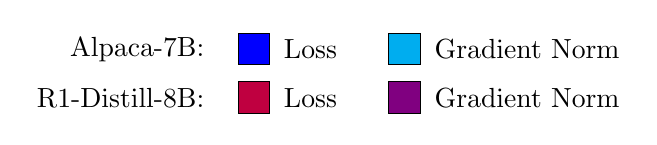
\begin{tikzpicture}
            \node[draw, fill=blue, minimum width=0.4cm, minimum height=0.4cm] (A) {};
            \node[left=0.3cm of A] {\modelalpaca:};
            \node[right=0.05cm of A] {Loss};

            \node[draw, fill=cyan, minimum width=0.4cm, minimum height=0.4cm, right=1.5cm of A] (B) {};
            \node[right=0.05cm of B] {Gradient Norm};

            \node[draw, fill=purple, minimum width=0.4cm, minimum height=0.4cm, below=0.2cm of A] (C) {};
            \node[left=0.3cm of C] {\modeldeepseek:};
            \node[right=0.05cm of C] {Loss};

            \node[draw, fill=violet, minimum width=0.4cm, minimum height=0.4cm, right=1.5cm of C] (D) {};
            \node[right=0.05cm of D] {Gradient Norm};
        \end{tikzpicture}
    }

    \caption{Fine-tuning of \modelalpaca and \modeldeepseek. Loss and gradient norm trends are shown separately for each model, along with a comparison of both losses. Figure and results from our work.}
    \label{fig:training_comparison}
\end{figure}

\begin{figure}[ht]
    \centering
    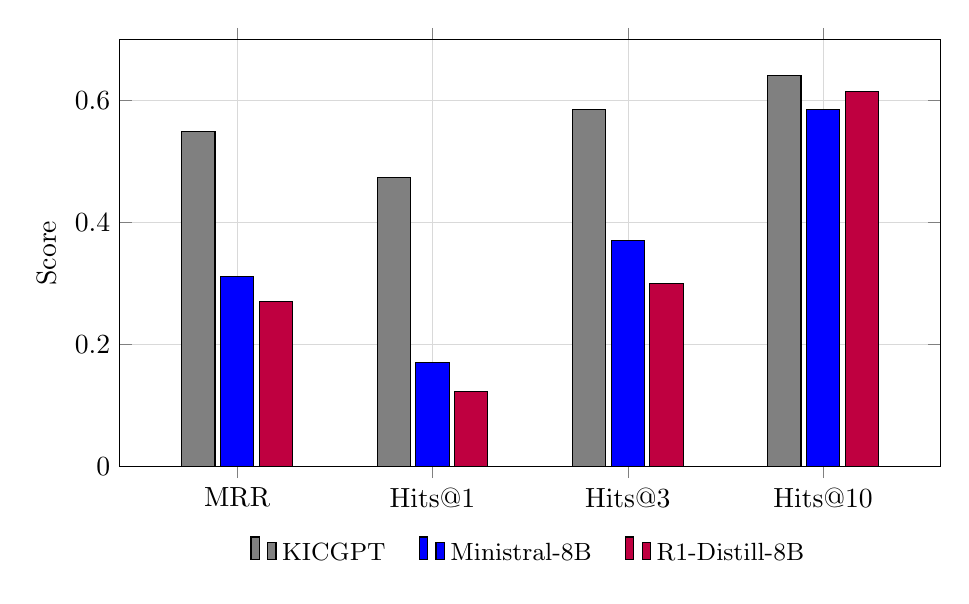
\begin{tikzpicture}
        \begin{axis}[
                ybar,
                bar width=12pt,
                symbolic x coords={MRR, Hits@1, Hits@3, Hits@10},
                xtick=data,
                ymin=0,
                ymax=0.7,
                ylabel={Score},
                width=12cm,
                height=7cm,
                grid=both,
                major grid style={line width=.2pt, draw=gray!30},
                minor grid style={draw=gray!10},
                enlarge x limits=0.2,
                % Legend placed below with spacing:
                legend style={
                        at={(0.5,-0.15)},
                        anchor=north,
                        /tikz/every even column/.append style={column sep=10pt},
                        legend columns=3,
                        draw=none, % Remove box
                        fill=none,
                        font=\small
                    }
            ]

            % Bars
            \addplot[fill=gray]   coordinates {(MRR,0.549)  (Hits@1,0.474)  (Hits@3,0.585)  (Hits@10,0.641)};
            \addlegendentry{KICGPT}
            \addplot[fill=blue]   coordinates {(MRR,0.3112) (Hits@1,0.1707) (Hits@3,0.3711) (Hits@10,0.5862)};
            \addlegendentry{\modelministral}
            \addplot[fill=purple] coordinates {(MRR,0.2700) (Hits@1,0.1233) (Hits@3,0.2994) (Hits@10,0.6145)};
            \addlegendentry{\modeldeepseek}

        \end{axis}
    \end{tikzpicture}
    \caption{Link Ordering Evaluation Metrics}
    \label{fig:link_ordering}
\end{figure}


\todo{Maybe shortly explain dataset?}
\todo{maybe QUICKLY intro metrics, however should be known already}

\subsection{Concise Model Summaries}

We use three models for our experiments:
Alpaca-7B~\cite{taori2023stanford} is a fine-tuned LLaMA 7B model designed for instruction-following tasks, trained on 52,000 examples generated via OpenAI’s text-davinci-003.
Ministral-8B-Instruct-2410~\cite{mistralai2024ministral8b} is an 8-billion-parameter model fine-tuned for instruction tasks, featuring a 128k context window and multilingual support, outperforming similar-sized models.
Compared to Alpaca, Ministral-8B benefits from a larger model size, an extended context window, and broader multilingual capabilities.
DeepSeek-R1-Distill-Llama-8B~\cite{deepseekai2025deepseekr1distillllama8b} is an 8-billion-parameter model distilled from DeepSeek-R1~\cite{guo2025deepseek}, focusing on reasoning and problem-solving, particularly excelling in math and code tasks.

All experiments were conducted on a system equipped with an NVIDIA RTX A5000 GPU with 24 GiB of VRAM, paired with an Intel Xeon W-1270P CPU running at 3.80 GHz and 64 GB of RAM.



\todo{Performance of KICGPT}

\todo{very unhappy with this, need to write somethign like this}
Following the procedure outlined in~\cref{sec:methodology}, we fine-tuned \modelalpaca on the CoDeX~\cite{safavi2020codex} dataset.
This process took 10 hours and 12 minutes, with the model converging as expected.
The training loss, shown in the leftmost plot of \cref{fig:training_comparison}, follows a bit noisy downward trend, while the gradient norm exhibits significant fluctuations but also trends downards over time.

Similarly, \modeldeepseek was fine-tuned under the same setup, with its training loss shown in the middle plot of \cref{fig:training_comparison}.
9h and 56 minutes.
The loss curve behaves similarly to \modelalpaca, confirming stable convergence, though the gradient norm remains similarly volatile throughout training.
The decreasing trend in gradient norm suggests that while updates remain unstable at each step, their overall magnitude diminishes as training progresses, indicating a gradual refinement of the optimization process.

The final comparison, shown in the rightmost plot of \cref{fig:training_comparison}, demonstrates that both models achieve nearly identical loss trajectories.
So we would expect them to perform similarly.

\todo{end of previous todo}

\todo{evaluations results}

52min alpa
56min r1

\begin{figure}[ht]
    \centering
    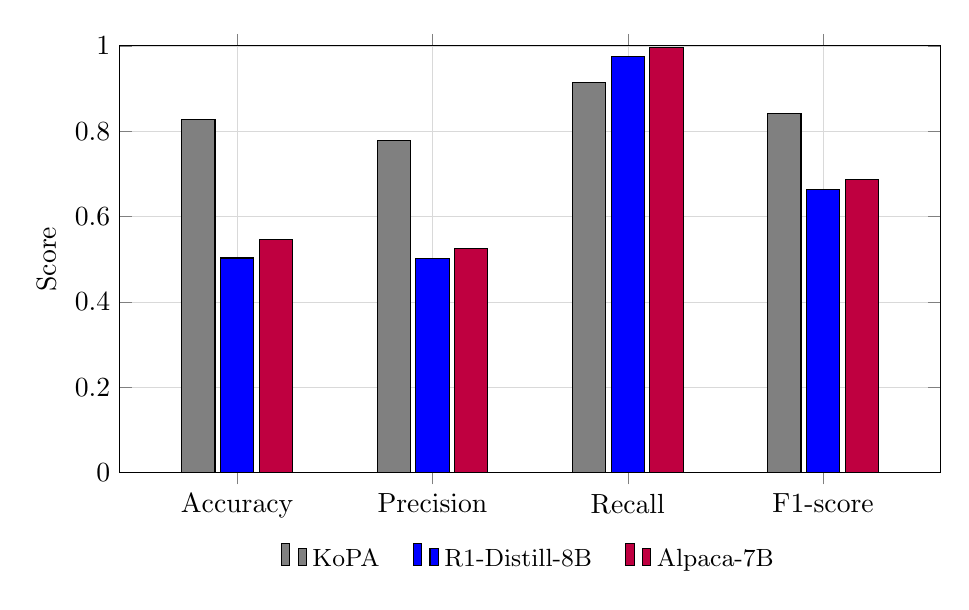
\begin{tikzpicture}
        \begin{axis}[
                ybar,
                bar width=12pt,
                symbolic x coords={Accuracy, Precision, Recall, F1-score},
                xtick=data,
                ymin=0,
                ymax=1,
                ylabel={Score},
                width=12cm,
                height=7cm,
                grid=both,
                major grid style={line width=.2pt, draw=gray!30},
                minor grid style={draw=gray!10},
                enlarge x limits=0.2,
                legend style={
                        at={(0.5,-0.15)},
                        anchor=north,
                        /tikz/every even column/.append style={column sep=10pt},
                        legend columns=3,
                        draw=none,
                        fill=none,
                        font=\small
                    }
            ]

            % Bars
            \addplot[fill=gray]   coordinates {(Accuracy,0.8274)  (Precision,0.7791)  (Recall,0.9141)  (F1-score,0.8411)};
            \addlegendentry{KoPA}

            \addplot[fill=blue]   coordinates {(Accuracy,0.5027) (Precision,0.5014) (Recall,0.9759) (F1-score,0.6625)};
            \addlegendentry{\modeldeepseek}

            \addplot[fill=purple] coordinates {(Accuracy,0.5465) (Precision,0.5245) (Recall,0.9962) (F1-score,0.6872)};
            \addlegendentry{\modelalpaca}
        \end{axis}
    \end{tikzpicture}
    \caption{CoDeX Performance Evaluation Metrics}
    \label{fig:codex_evaluation}
\end{figure}

% ---------------------------------------------------------
%
% DISCUSSION
%
% ---------------------------------------------------------


\section{Discussion}\label{sec:discussion}
\todo{TBD, only do if there is actual deeper meaning otherwise fuse with experiments}

\todo{Interpret the results in a deeper way:
    - Why did certain methods do better?
    - Mention any error analysis or interesting observations.
}

The link prediction performance of \modeldeepseek, \modelministral, and ChatGPT varies due to differences in inference behavior, decoding strategies, and instruction adherence.

\modeldeepseek struggled to follow formatting constraints despite explicit prompts. It often produced verbose reasoning before generating answers and self-trimmed responses, sometimes omitting correct entities. This suggests a pretraining bias favoring exhaustive analysis, which conflicted with structured output requirements. Its decoding strategy prioritized information compression, reducing MRR and Hits@1 scores. The few-shot prompting setup may have worsened its tendency to "overthink," making precise, structured outputs harder to achieve.

\modelministral performed better at instruction adherence and structured output than \modeldeepseek. It balanced reasoning depth with clarity but lacked ChatGPT's reranking optimizations, leading to lower MRR and weaker top-ranked predictions. While it ranked entities more consistently, its Hits@10 score lagged slightly, indicating fewer retrieved correct entities overall. Nonetheless, its superior instruction-following made it more effective than \modeldeepseek for structured tasks.

ChatGPT outperformed both models, excelling in instruction adherence and ranking precision due to RLHF and advanced reranking heuristics. It avoided \modeldeepseek's verbosity and \modelministral's retrieval inefficiencies, yielding higher MRR, Hits@1, and Hits@3 scores. Its ability to dynamically contextualize information in few-shot settings further improved entity predictions, making it the most effective model for knowledge graph completion.

% ---------------------------------------------------------
%
% CONCLUSION
%
% ---------------------------------------------------------


\section{Conclusion and Future Work}\label{sec:conclusion-and-future-work}
\todo{TBD otherwise leave out}
\todo{Summarize the key findings and how they link back to your problem statement. Suggest improvements or next steps (e.g., new dataset, advanced fusion technique, or GNN-based approach). Highlight what you learned and what remains challenging.}

\bibliography{main}

\end{document}
